\documentclass[margin=1mm]{standalone}
\usepackage{tikz}

\tikzset{
  double arrow/.style args={#1 colored by #2 and #3}{
    -stealth,line width=#1,#2, % first arrow
    postaction={draw,-stealth,#3,line width=(#1)/3,
                shorten <=(#1)/3,shorten >=2*(#1)/3}, % second arrow
  }
}

\begin{document}
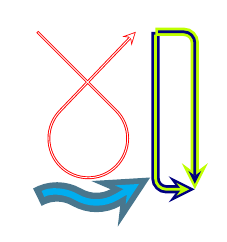
\begin{tikzpicture}
		
		\draw[double arrow=1pt colored by red and white]
		(0,2) -- (1,1) arc(45:-360+45+90:.5) -- (1.25,2);

		\draw[double arrow=3pt colored by blue!50!black and lime,rounded corners]
		(1.5,2)  |- (2,0);

		\draw[double arrow=3pt colored by lime and blue!50!black,rounded corners]
		(1.5,2)  -| (2,0);
		
		\draw[double arrow=7pt colored by cyan!50!black and cyan]
		(0,-.1) arc(120:60:.5) arc(-120:-60:.5) -- ++(30:.5);
		
		
\end{tikzpicture}
\end{document}
